\chapter{Johnson-Rauschen}
% ----
In diesem Kapitel wird das Johnson-Rauschen in Widerständen untersucht.\\ 
Das Johnson-Rauschen entsteht durch die thermische Fluktuation der Ladungsträger in einem ohmschen Widerstand und führt zu zufälligen Spannungsschwankungen über dem Widerstand. Diese Spannungsschwankungen sind proportional zum Widerstand $R$, sowie seiner Temperatur $T$ und werden durch die Nyquist-Beziehung\cite{paper} beschrieben:
\begin{equation}
    \langle V^2 \rangle = 4 k_B T R \Delta f, \label{equ:nyquist}
\end{equation}
wobei $\langle V^2 \rangle$ die mittlere quadratische (MS \enquote{mean square}) Spannung, $k_B$ die Boltzmann-Konstante und $\Delta f$ die effektive Bandbreite des Messsystems ist.
% ----
\section{Visualisierung des Johnson-Rauschens}
% ----
Zunächst wird das Johnson-Rauschen visuell dargestellt. Da es nur eine sehr geringe Signalstärke aufweist, wird das Rauschsignal mit einem speziellen Vorverstärker (\cref{fig:johnson_lle}), einem nicht-invertierenden Operationsverstärker eingebaut in die \enquote{\texttt{Low-Level electronics}-Box} (LLE), verstärkt. \\
\begin{figure}[h]
    \centering
    \subcaptionbox{Vorverstärker der LLE-Box}{\includegraphics[keepaspectratio, width=5cm]{figs/schalt_amplifier.png}}
    \subcaptionbox{LLE-Box}{\includegraphics[keepaspectratio, width=7cm]{figs/johnson_lle.png}}
    \caption{Schaltpläne zur Verstärkung des Johnson-Rauschens~\cite{praktikum4_atome}}\label{fig:johnson_lle}
\end{figure}

Die Verstärkerelektronik besteht aus zwei Stufen, sodass eine Gesamtverstärkung von $G_1 = 600$ erreicht wird. Das verstärkte Rauschsignal gelangt hiernach an die HLE-Box, einem Bandpass welcher gezielt die relevanten Frequenzbereiche herausfiltert und einem einstellbaren Verstärker (\enquote{Gain}), und wird schließlich auf dem Oszilloskop dargestellt (\cref{fig:johnson_aufbau}).
\begin{figure}[h]
    \centering
    \subcaptionbox{Schaltplan zur Messung des \\ Johnson-Rauschens~\cite{praktikum4_atome}}{\includegraphics[keepaspectratio,width=0.48\textwidth]{figs/johnson_hle.png}}
    \subcaptionbox{Johnson-Rauschen bei $T = \qty{21.4\pm 0.2}{\degreeCelsius}$;\\ $T$/div$=\qty{500}{\micro\second}$; $V$ / div $=\qty{800}{\milli\volt}$;\\ Triggerlevel $\approx 0$; Eingangsimpedanz am Oszilloskop:$\qty{1}{\mega\ohm}$}{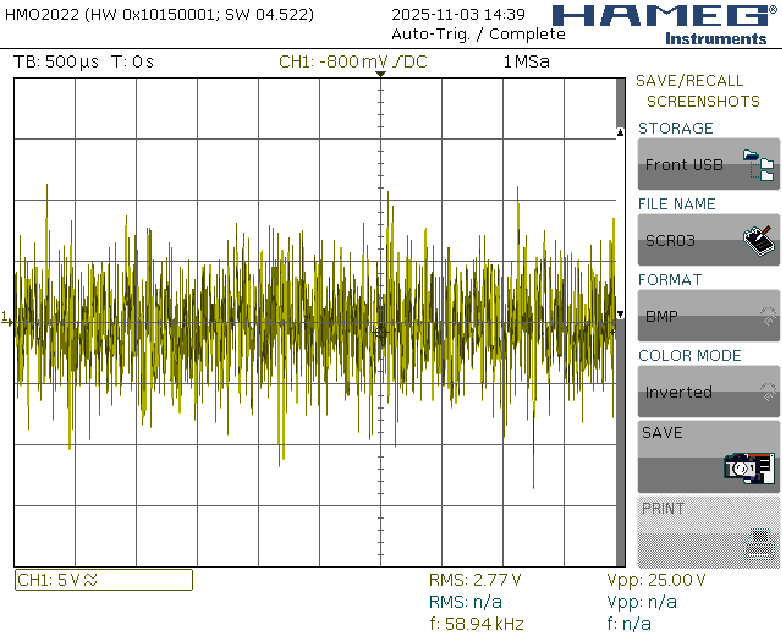
\includegraphics[keepaspectratio,width=0.48\textwidth]{images/johnson_oszi.pdf}}
    \caption{Visualisierung des Johnson-Rauschens}\label{fig:johnson_aufbau}
\end{figure}
\subsection{Beobachtung des Johnson-Rauschens}
Die Widerstände der LLE-Box werden auf $R_{\mathrm{in}} = \qty{100}{\kilo\ohm}$ und $R_f = \qty{1}{\kilo\ohm}$ und die Grenzfrequenzen der HLE-Box auf $f_{\mathrm{LP}} = \qty{10}{\kilo\hertz}$ und $f_{\mathrm{HP}} = \qty{1}{\kilo\hertz}$ eingestellt.\cite{praktikum4_atome}\\
Auf dem Oszilloskop ist das Rauschsignal als zufällige Spannungsschwankungen um den Mittelwert von Null zu erkennen (\cref{fig:johnson_aufbau}).
% ----
 \subsection{Messung des Johnson-Rauschens mit der HLE-Box}
% ----
Nun wird die HLE-Box wie in \cref{fig:johnson_hle_messung} an einen Multiplier im \emph{AxA}-Modus geschlossen.\\
Hierbei wird das Rauschsignal am Ausgang der HLE-Box gemäß
\begin{equation}
    V_{\mathrm{out}} = \frac{\overline{V_{\mathrm{in}}^2(t)}}{\qty{10}{\volt}}\label{equ:multiplier}
\end{equation}
quadriert. Das Ausgangssignal des Multipliers wird intern durchgeschleift und über eine einstellbare Zeitkonstante $\tau=\qty{1}{\second}$ gemittelt. 
\begin{figure}[h]
    \centering
    \includegraphics[width=0.6\textwidth]{figs/johnson_hle_and_dmm.png}
    \caption{Schaltplan zur Messung des Johnson-Rauschens mit der HLE-Box~\cite{praktikum4_atome}}\label{fig:johnson_hle_messung}
\end{figure}

Um die Funktionsweise des Multipliers zu überprüfen wird zunächst das Monitor-Signal des Multipliers mit dem Kanal 2 des Oszilloskops verbunden. Dieses Signal entspricht dem quadrierten Eingangssignal des Multipliers, also dem quadrierten Rauschsignal der HLE-Box. An Kanal 1 wird das Ausgangssignal der HLE-Box, also das Johnson-Rauschen, geschlossen und der XY-Modus des Oszilloskops eingerichtet. Hierbei wurde geachtet, dass die Ausgabe auf dem Digitalmultimeter (DMM) nur Werte zwischen $\SIrange{0.6}{1.2}{\volt}$ anzeigt, da nur in deisem Bereich die Ausgangssignale stabil und linear zum Eingangsrauschen sind.\\
In \cref{fig:johnson_xy_mode} ist die XY-Darstellung des Johnson-Rauschens gegen das quadrierte Signal des Multipliers zu sehen. Es zeigt sich, dass das Ausgangssignal des Multipliers proportional zum Quadrat des Eingangssignals ist, was die Funktionsweise des Multipliers bestätigt.
\begin{figure}[h]
    \centering
    \includegraphics[keepaspectratio, width=0.6\textwidth]{images/johnson_multiplier.png}
    \caption{XY-Darstellung des Johnson-Rauschens und des quadrierten Signals am Monitor-Ausgang des Multipliers}\label{fig:johnson_xy_mode}
\end{figure}
% ----
\section[Johnson-Rauschen (Widerstand)]{Abhängigkeit des Johnson-Rauschens von Widerstand}
% ----
Um den linearen Zusammenhang zwischen dem Johnson-Rauschen und dem Widerstand gemäß Nyquist-Formel (\cref{equ:nyquist}) zu untersuchen, wird das Ausgangssignal des Multipliers für verschiedene Widerstandswerte $R$ gemessen. Hierzu werden die Widerstände der LLE-Box auf $R_{\mathrm{in}} = R$ und $R_f = \qty{1}{\kilo\ohm}$ eingestellt. Die Grenzfrequenzen der HLE-Box bleiben unverändert bei $f_{\mathrm{LP}} = \qty{10}{\kilo\hertz}$ und $f_{\mathrm{HP}} = \qty{1}{\kilo\hertz}$\\
Die Messung wurde bei Raumtemperatur $T = \qty{21.4 \pm 0.2}{\degreeCelsius} = \qty{294.55 \pm 0.2}{\kelvin}$ durchgeführt. Die gemessenen Ausgangsspannungen des Multipliers $V_{\mathrm{out}}$ sind in \cref{tab:johnson_widerstand} aufgelistet.
\begin{table}[h!]
    \centering
    \begin{tabular}{
        S[table-format=7.0]
        @{$\,\pm\,$}
        S[table-format=5.2]|
        S[table-format=4.0]
        S[table-format=1.3(1)]
        S[table-format=3.2(3)]}
    \toprule
    \multicolumn{2}{c|}{$R$ / $\Omega$} &
    \multicolumn{1}{c}{$G_2$} &
    \multicolumn{1}{c}{$V_{\mathrm{DMM}}$ / V} &
    \multicolumn{1}{c}{$V_J^2$ / V$^2\cdot10^{-12}$} \\
    \midrule
      1 & 0.01     & 2000 & 1.003 \pm 0.005 & 6.96 \pm 0.04 \\
     10 & 0.10     & 2000 & 1.004 \pm 0.005 & 6.97 \pm 0.04 \\
    100 & 1.00     & 2000 & 1.026 \pm 0.005 & 7.12 \pm 0.04 \\
   1000 & 10.00    & 1500 & 0.714 \pm 0.005 & 8.81 \pm 0.06 \\
  10000 & 100.00   & 1000 & 0.924 \pm 0.005 & 25.68 \pm 0.14 \\
 100000 & 1000.00  & 400  & 0.840 \pm 0.005 & 145.78 \pm 0.87 \\
1000000 & 10000.00 & 300  & 0.880 \pm 0.005 & 271.48 \pm 1.54 \\
    \bottomrule
    \end{tabular}
    \caption{Messwerte der Johnson-Rauschspannung $V_J^2$ für verschiedene Widerstände $R$ bei Verstärkung $G_2$. Für $\Delta R$ wurde ein Fehler von $\qty{1}{\percent}$ angenommen.}
    \label{tab:johnson_widerstand}
\end{table}
Um störende Einflüsse, z.B. Eigenrauschen nachgeschalteter Verstärkerstufen, zu minimieren, wurde das Verstärkerverhältnis $G_2$ als fehlerfrei angenommen, während für die Spannung am DMM eine konstante Unsicherheit von $\Delta U_{\mathrm{DMM}}=\qty{0.005}{\volt}$ aufgrund der Fluktuation der Werte beim ablesen berücksichtigt wurde.\\
Die Werte für die Verstärkung $G_2$ sind so gewählt, dass die Ausgangsspannung des Multipliers stets im linearen Bereich zwischen $\SI{0.6}{\volt}$ und $\SI{1.2}{\volt}$ liegt.\\
Der vom DMM ausgegebene Wert hängt vom quadratischen Mittelwert der Rauschspannung am Eingang des Multipliers ab. Um die Johnson-Rauschspannung $V_J^2$ zu berechnen, wird der gemessene Wert mit den Verstärkungsfaktoren und dem Divisor des Multipliers skaliert:
\begin{align}
    V_{\mathrm{DMM}} &= \frac{\overline{V_J^2}\cdot (600\cdot G_2)^2}{\qty{10}{\volt}}\label{equ:johnson_dmm}\\
    \Leftrightarrow V_J^2 &= V_{\mathrm{DMM}} \cdot \SI{10}{\volt} \cdot \frac{1}{G_2^2}
\end{align}
Um zusätzliche Rauschkomponenten zu isolieren, die nicht als Johnson-Rauschen klassifiziert werden können, und unter der Annahme, dass $\overline{V_J^2}$ zusätzliche Störkomponenten enthält, wird \cref{equ:johnson_dmm} um eine  weitere Komponente erweitert:
\begin{equation}
    V_{DMM} = \frac{\overline{V_J^2}(600\cdot G_2)}{\qty{10}{\volt}} = \frac{\overline{V_J'^2 + V_N^2}(600\cdot G_2)}{\qty{10}{\volt}}
\end{equation}
wobei es keine Korrelation zwischen dem Johnson-Rauschen $V_J'$ und dem zusätzlichen Rauschen $V_N$ gibt, da beide in verschiedenen Komponenten entstehen ($V_J'$ im Widerstand, $V_N$ im Verstärker). Somit gilt:
\begin{equation}
    \overline{V_J^2} =\overline{V_J'^2 + V_N^2} = \overline{V_J'^2} + \overline{V_N^2}
\end{equation}
und man erhält die lineare Beziehung:
\begin{equation}
    \overline{V_J^2(R)} = \frac{V_{\mathrm{DMM}}\cdot \qty{10}{\volt}}{(600\cdot G_2)^2} = \overline{V_J'^2(R)} + \overline{V_N^2} = 4 k_B T \Delta f R + \overline{V_N^2} \label{equ:johnson_linear}
\end{equation}
Durch eine lineare Regression nach \cref{equ:johnson_linear} kann nun das Johnson-Rauschen von dem zusätzlichen Rauschen getrennt und das Rauschverhalten in Abhängigkeit des Widerstands dargestellt werden.\\
Dafür wird in \cref{fig:johnson_widerstand_linear} und \cref{fig:johnson_widerstand_log} die gemessene Johnson-Rauschspannung $V_J^2$ gegen den Widerstand $R$ einmal linear und einmal halblogarithmisch aufgetragen.\\
An die Messwerte wird eine Anpassungsgerade der Form:
\begin{equation*}
    V_J^2(R) = m \cdot R + b
\end{equation*}
gelegt, wobei die Steigung $m$ und der Achsenabschnitt $b$ durch die lineare Regression bestimmt werden.\\
\begin{figure}[h]
    \centering
    \includegraphics[keepaspectratio, width=0.7\linewidth]{plots/johnson_rauschen_widerstand_norm_residuen.pdf}
    \caption{Graphische Darstellung der Widerstandsabhängigkeit des Johnson-Rauschens $V_J^2$ mit linearer Regression nach \cref{equ:johnson_linear} und normierten Residuen.\\(lineare Darstellung)}\label{fig:johnson_widerstand_linear}
\end{figure}
\begin{figure}[h]
    \centering
    \includegraphics[keepaspectratio, width=0.7\linewidth]{plots/johnson_rauschen_widerstand_norm_residuen_log.pdf}
    \caption{Graphische Darstellung der Widerstandsabhängigkeit des Johnson-Rauschens $V_J^2$ mit linearer Regression nach \cref{equ:johnson_linear} und normierten Residuen.\\(halblogarithmische Darstellung)}\label{fig:johnson_widerstand_log}
\end{figure}
Zur überprüfung der Güte der linearen Regression wurden im Anschluss an die Auslgeichrechnung die Residuen berechnet und aufgetragen. Diese geben an, wie stark einzelne Messwerte von der Anpassungsgeraden abweichen.\\
Für jeden Messpunkt gilt:
\begin{equation}
    r_i = y_i -(mR_i + b)
\end{equation}
wobei $y_i = V_{J,i}^2$ die gemessenen Werte und $(mR_i+b)$  die durch den lineare Anpassung bestimmten Modellwerte sind. Ein zufälliges Streuen um den Wert Null zeigt, dass das Modell die Messdaten gut beschreibt.\\
Zur weiteren Bewertung der Anpassungsgüte wurden die normalisierten Residuen berechnet.\\
Dabei wird jedes Residuum durch seine kombinierte Unsicherheit geteilt, um seine statistische Signifikanz zu bewerten:
\begin{equation}
    r_i^{\mathrm{norm}} = \frac{r_i}{\sigma_{r,i}}
\end{equation}
Die Unsicherheit wird hier in guter Näherung $\sigma_{r,i}=\sigma_{yi}$ angenommen, da die Fitunsicherheit klein gegenüber dem Messfehler ist. Die normierten Residuen sollten im Idealfall zufällig um Null streuen und im Bereich $-2\leq r_i^{\mathrm{norm}}\leq 2$ liegen, um die Richtigkeit des Modells und realistische Einschätzung der Messfehler zu bestätigen.
\vspace{0.2cm}

Anhand der Messpunkte wird deutlich, dass für große Widerstände die Werte für $V_J^2$ abflachen. Aus diesem Grund wurde die Anpassung mit 3 Messsätzen durchgeführt welche folgende Fitparameter liefern:
\begin{itemize}
    \item Mit allen Messwerten:
    \begin{itemize}
        \item $m = \qty{3.168(15)e-16}{\volt\squared\per\ohm}$
        \item $b = \qty{7.477(19)e-12}{\volt\squared}$
        \item $\chi_{\mathrm{red}}^2 = 5759.29$
    \end{itemize}
    \item ohne den letzten Messwerte:
    \begin{itemize}
        \item $m = \qty{1.524(7)e-15}{\volt\squared\per\ohm}$
        \item $b = \qty{7.052(19)e-12}{\volt\squared}$
        \item $\chi_{\mathrm{red}}^2 = 218.89$
    \end{itemize}
    \item ohne die letzten beiden Messwerte:
    \begin{itemize}
        \item $m = \qty{1.872(14)e-15}{\volt\squared\per\ohm}$
        \item $b = \qty{6.950(19)e-14}{\volt\squared}$
        \item $\chi_{\mathrm{red}}^2 = 0.11$
    \end{itemize}
\end{itemize}
Die Steigung $m$ entspricht dem Produkt $4k_B T\Delta f$, wobei die Bandbreite im vorherigen Teil auf $\Delta f = \qty{11396.7 \pm 463.4}{\hertz}$ bestimmt wurde.\\
Die Boltzmann Konstante kann nun aus der Steigung berechnet werden zu:
\begin{equation*}
  k_B = \frac{m}{4T\Delta f}
  = \left\{
  \begin{array}{@{}l@{\quad}l@{}}
    \qty{2.359(97)e-23}{\joule\per\kelvin} & \text{,für alle Messwerte},\\[4pt]
    \qty{1.135(46)e-22}{\joule\per\kelvin} & \text{,ohne den letzten Messwert},\\[4pt]
    \qty{1.394(58)e-22}{\joule\per\kelvin} & \text{,ohne die letzten beiden Messwerte.}
  \end{array}
  \right.
\end{equation*}
Alle diese Werte weichen stark vom Literaturwert $k_B^{\mathrm{lit}} = \qty{1.380649e-23}{\joule\per\kelvin}$\cite{NIST} ab und er liegt auch in keinem der Fehlerbereiche. Jedoch ist beachtlich, dass der ermittelte Wert der Boltzmann Konstanten unter Beachtung aller Messwerte näher am Literaturwert liegt, als die beiden Messsätze ohne letzten 1 bzw. 2 Punkte, obwohl die Güte der Anpassungsgeraden bei diesen weit höher sind.\\
Neben möglich Fehlerhafter Messung und Störungen (die Werte $V_{\mathrm{DMM}}$ wurden schon allein durch Lautstärke beeinflusst) könnte ein weiterer Faktor der Temperaturunterschied der Widerstände sein. So heizen sich die kleineren Widerstände mehr auf, wodurch der angenommene Temperaturwert von $T = \qty{21.4\pm 0.2}{\degreeCelsius}$ zu gering geschätzt ist. Dies sieht man gut durch die Anpassungsgerade, welche einen weitaus steileren Anstieg ausweist, als wenn der Wert für $R=\qty{1}{\mega\ohm}$ berücksichtigt wird. Ein weiteres Indiz hierfür ist der \enquote{abgeflachte} Wert für eben diesen Widerstand. Wird dieser Widerstand mitberücksichtig, dann gleicht das den Temperaturanstieg für die kleineren Widerstände (wenn auch nur geringfügig) aus, wodurch der Wert für die Boltzmannkonstante besser angenähert wird.\\
Dies könnte mit einer Messung für Widerstände zwischen $\SIrange{100}{999}{\kilo\ohm}$ bestätigt oder widerlegt werden. 
% ----
\section[Johnson-Rauschen (Bandbreite)]{Abhängigkeit des Johnson-Rauschens von der Bandbreite}
Analog zum Widerstand beschreibt die Nyquist-Formel \cref{equ:nyquist} die lineare Abhängigkeit des Johnson-Rauschens von der Bandbreite. Zur Untersuchung dieser Beziehung wird an der HLE-Box verschiedene Hoch- und Tiefpasskonfigurationen eingestellt, um die Bandbreite zu variieren. Zur Reduzierung äußerer Einflüsse und externer Rauschquellen wurde ein $R = \qty{1}{\mega\ohm}$ Widerstand verwendet. Die resultierende Ausgangsspannung wird vermessen (\cref{tab:johnson_bandbreite}) und gegen die Bandbreite aufgetragen \cref{fig:johnson_bandbreite}.
\begin{table}[h!]
    \centering
    \begin{tabular}{
        S[table-format=4.0]
        @{$\,\pm\,$}
        S[table-format=2.0]|
        S[table-format=6.0]
        @{$\,\pm\,$}
        S[table-format=4.0]|
        S[table-format=3.0]|
        S[table-format=1.3(2)]|
        S[table-format=5.0]
        @{$\,\pm\,$}
        S[table-format=4.0]|
        S[table-format=3.1(2)]}
    \toprule
    \multicolumn{2}{c|}{$f_h$ / Hz} &
    \multicolumn{2}{c|}{$f_l$ / Hz} &
    \multicolumn{1}{c|}{$G$} &
    \multicolumn{1}{c|}{$U_{\mathrm{DMM}}$ / V} &
    \multicolumn{2}{c|}{$\Delta f$ / Hz} &
    \multicolumn{1}{c}{$V_J^2$ / V$^2\cdot 10^{-12}$} \\
    \midrule
     100 & 1  & 100000 & 1000 & 300 & 0,876 \pm 0,010 & 99900 & 1000 & 270,5 \pm 3,1 \\
     100 & 1  & 33000  & 330  & 300 & 0,690 \pm 0,010 & 32900 & 330  & 213,0 \pm 3,1 \\
     100 & 1  & 10000  & 100  & 400 & 0,742 \pm 0,010 & 9900  & 100  & 128,7 \pm 1,7 \\
     100 & 1  & 3300   & 33   & 600 & 0,705 \pm 0,010 & 3200  & 33   & 54,4  \pm 0,8 \\
     300 & 3  & 3300   & 33   & 600 & 0,655 \pm 0,010 & 3000  & 33   & 50,6  \pm 0,8 \\
     300 & 3  & 10000  & 100  & 400 & 0,719 \pm 0,010 & 9700  & 100  & 124,8 \pm 1,7 \\
     300 & 3  & 33000  & 330  & 300 & 0,683 \pm 0,010 & 32700 & 330  & 210,8 \pm 3,1 \\
     300 & 3  & 100000 & 1000 & 300 & 0,865 \pm 0,010 & 99700 & 1000 & 267,1 \pm 3,1 \\
    1000 & 10 & 100000 & 1000 & 300 & 0,879 \pm 0,010 & 99000 & 1000 & 271,4 \pm 3,1 \\
    1000 & 10 & 33000  & 330  & 300 & 0,692 \pm 0,010 & 32000 & 330  & 213,5 \pm 3,1 \\
    1000 & 10 & 10000  & 100  & 400 & 0,734 \pm 0,010 & 9000  & 100  & 127,5 \pm 1,7 \\
    1000 & 10 & 3300   & 33   & 600 & 0,701 \pm 0,010 & 2300  & 35   & 54,1  \pm 0,8 \\
    \bottomrule
    \end{tabular}
    \caption{Messwerte zur Rauschleistungsanalyse bei variierender Bandbreite: obere und untere Grenzfrequenzen $f_h$ und $f_l$, Verstärkung $G$, gemessene Spannung $U_{\mathrm{DMM}}$, Frequenzdifferenz $\Delta f$ und zugehörige Johnson-Rauschspannung $V_J^2$.}\label{tab:johnson_bandbreite}
\end{table}
\begin{figure}[h]
    \centering
    \includegraphics[width=0.7\textwidth]{plots/johnson_rauschen_bandbreite.pdf}
    \caption{Grafische Darstellung der Bandbreitenabhängigkeit des Johnson-Rauschens $V_J^2$ mit linearer Regression}
    \label{fig:johnson_bandbreite}
\end{figure}
Zuerst fällt auf, dass sich bei der Auswahl der Messpunkte für die Bandbreite ein Denkfehler eingeschlichen hat, sodass die Werte in Gruppen \enquote{verklumpt} anstatt gleichmäßig verteilt sind.\\
Die lineare Anpassung der Form:
\begin{equation*}
    V_J^2(\Delta f) = m\cdot \Delta f + b
\end{equation*}
liefert folgende Parameter:
\begin{align*}
    m &= \qty{2.459(18)e-15}{\volt\squared\per\ohm}\\
    b &= \qty{5.773(43)}{\volt\squared}\\
    \chi_{\mathrm{red}}^2 &= 490.31
\end{align*}
Die Steigung $m$ entspricht dem Produkt $4k_B T \Delta f$, wobei die Temperatur auch hier auf $T = \qty{21.4 \pm 0.2}{\degreeCelsius}$ gemessen wurde.\\
Hieraus lässt sich die Boltzmann Konstante ermitteln zu:
\begin{equation*}
    k_B = \frac{m}{4T\Delta f} = \qty{2.087(26)e-24}{\joule\per\kelvin}
\end{equation*}
Auch hier weicht der ermittele Wert stark vom Literaturwert ab.\\
Dies lässt sich, abgesehen von fehlerhafter Messung und den im vorherigen Abschnitt benannten gründen, durch nicht ausreichend Ausgebreitete Messpunkte begründen, wodurch im Grunde genommen nur eine Anpassung mit 4 Werte-Cluster durchgeführt wird. Auch wurde, wie an \cref{fig:johnson_bandbreite} ersichtlich ein zu geringer Fehler angenommen, wodurch entsprechend auch die Güte der Anpassung abnimmt.